%%\documentclass[a4paper,12pt,oneside]{llncs}
\documentclass{book}
%\usepackage[right=2cm,left=3cm,top=2cm,bottom=2cm,headsep=0cm]{geometry}

%%%%%%%%%%%%%%%%%%%%%%%%%%%%%%%%%%%%%%%%%%%%%%%%%%%%%%%%%%%
%% Juego de caracteres usado en el archivo fuente: UTF-8
\usepackage{ucs}
\usepackage[utf8x]{inputenc}

%%%%%%%%%%%%%%%%%%%%%%%%%%%%%%%%%%%%%%%%%%%%%%%%%%%%%%%%%%%
%% Juego de caracteres usado en la salida dvi
%% Otra posibilidad: \usepackage{t1enc}
\usepackage[T1]{fontenc}

%%%%%%%%%%%%%%%%%%%%%%%%%%%%%%%%%%%%%%%%%%%%%%%%%%%%%%%%%%%
%% Ajusta maergenes para a4
\usepackage{a4wide}

%%%%%%%%%%%%%%%%%%%%%%%%%%%%%%%%%%%%%%%%%%%%%%%%%%%%%%%%%%%
%% Uso fuente postscript times, para que los ps y pdf queden y pequeños...
\usepackage{times}

%%%%%%%%%%%%%%%%%%%%%%%%%%%%%%%%%%%%%%%%%%%%%%%%%%%%%%%%%%%
%% Posibilidad de hipertexto (especialmente en pdf)
\usepackage{hyperref}

%%%%%%%%%%%%%%%%%%%%%%%%%%%%%%%%%%%%%%%%%%%%%%%%%%%%%%%%%%%
%% Graficos 
\usepackage{graphics,graphicx}

%%%%%%%%%%%%%%%%%%%%%%%%%%%%%%%%%%%%%%%%%%%%%%%%%%%%%%%%%%%
%% Ciertos caracteres "raros"...
\usepackage{latexsym}

%%%%%%%%%%%%%%%%%%%%%%%%%%%%%%%%%%%%%%%%%%%%%%%%%%%%%%%%%%%
%% Matematicas aun más fuertes (american math dociety)
\usepackage{amsmath}

%%%%%%%%%%%%%%%%%%%%%%%%%%%%%%%%%%%%%%%%%%%%%%%%%%%%%%%%%%%
\usepackage{multirow} % para las tablas
\usepackage[spanish,es-tabla]{babel}

%%%%%%%%%%%%%%%%%%%%%%%%%%%%%%%%%%%%%%%%%%%%%%%%%%%%%%%%%%%
%% Fuentes matematicas lo mas compatibles posibles con postscript (times)
%% (Esto no funciona para todos los simbolos pero reduce mucho el tamaño del
%% pdf si hay muchas matamaticas....
\usepackage{mathptm}

%%% VARIOS:
\usepackage{slashbox}
\usepackage{verbatim}
\usepackage{array}
\usepackage{listings}
\usepackage{multirow}

%% MARCA DE AGUA
%% Este package de "draft copy" NO funciona con pdflatex
%%\usepackage{draftcopy}
%% Este package de "draft copy" SI funciona con pdflatex
%%%\usepackage{pdfdraftcopy}
%%%%%%%%%%%%%%%%%%%%%%%%%%%%%%%%%%%%%%%%%%%%%%%%%%%%%%%%%%%
%% Indenteacion en español...
\usepackage[spanish]{babel}
\usepackage{Estilos/Apuntes}
\usepackage[svgnames,x11names,table]{xcolor}
\usepackage{listings}
% Para escribir código en C
% \begin{lstlisting}[language=C]
% #include <stdio.h>
% int main(int argc, char* argv[]) {
% puts("Hola mundo!");
% }
% \end{lstlisting}


\title{Documentación CPD}
\author{Jesús Rodríguez Heras\\Elías Makdad Khamlichi\\Juan de la Cruz Caravaca Guerrero\\Francisco Javier Gómez Coronil}

\begin{document}
	\maketitle
	\thispagestyle{empty}
	\newpage
	
	\tableofcontents
	\newpage
	
	%%\listoftables
	%%\newpage
	
	%%\listoffigures
	%%\newpage
	
	%%%% REAL WORK BEGINS HERE:
	
	%%Configuracion del paquete listings
	\lstset{language=bash, numbers=left, numberstyle=\tiny, numbersep=10pt, firstnumber=1, stepnumber=1}

\chapter{Documentación}
\section{Descripción funcional}
Este programa tiene la finalidad de ser usado para administrar un centro educativo, el cual tiene una serie de administradores (director o jefe de estudios), profesores y alumnos. De todos ellos se guardará la información más relevante para el sistema en distintos ficheros que finalmente configurarán una base de datos en la cual tendremos concentrado a todo el personal del centro.\\
Al iniciar el programa se realiza el volcado de memoria de los ficheros, guardados en disco, a las estructuras creadas por el programa en memoria principal, lo que deja estructurado el sistema en dicha memoria principal.\\
Después de realizar los cambios necesarios en el programa, este vuelve a guardar los datos existentes en la memoria principal en los ficheros del disco.

\section{Descomposición del problema}
El problema (programa) ha sido descompuesto en 3 partes bien diferenciadas tales como es el sistema de volcado de memoria, el perfil administrador y el perfil profesor.\\
Cada uno de las partes ha sido implementada en un módulo distinto y todo se ha enlazado de forma que haya una mayor cohesión en el módulo y el menor acoplamiento posible entre los mismos.

\section{Documentación por módulo}
\subsection{Módulo 1: Ficheros}{
Este módulo se encarga del volcado de datos del disco a memoria principal y viceversa (al terminar el programa).\\
Contiene las estructuras (registros) mediante los cuales podremos identificar cada campo de los usuarios pedidos en el sistema.\\
También incorpora la funcionalidad de acceso al sistema que identifica a un usuario como administrador o profesor y les muestra sus funcionalidades disponibles.\\
Está implementado con una serie de funciones declaradas como \texttt{static} (para que solo puedan ser utilizadas en este módulo) y contiene unas variables globales que contabilizarán el número actual de registros presentes en el sistema.\\
Además, guarda una variable global con el identificador de usuario actual en el sistema para que, por ejemplo, no se pueda eliminar a sí mismo.\\
Estas variables globales nos darán información sobre cuantos usuarios, alumnos, materias, matrículas, calificaciones, faltas y horarios hay presentes en el sistema.
}
\subsection{Módulo 2: Administrador}{
Este módulo se encarga de gestionar todas las funciones disponibles para un administrador. Está compuesto por una serie de funciones declaradas como \texttt{static} que se encargan de todo el proceso.
}
\subsection{Módulo 3: Profesor}{
Este módulo se encarga de gestionar todas las funciones disponibles para un profesor. Está compuesto por una serie de funciones declaradas como \texttt{static} que se encargan de todo el proceso.
}

\section{Proceso de instalación}
El proceso de instalación consiste en tener el programa, ubicarlo en la carpeta deseada y abrirlo con doble click.\\
Una vez hecho esto, el programa generará los archivos necesarios para su ejecución tales como los ficheros que deberán ser completados a mano por el usuario una vez se haya ejecutado dicho programa.

\section{Ejecución del programa}
Una vez ejecutado el programa se realiza el volcado de información de los ficheros, guardados en disco, a las estructuras creadas por el programa en memoria principal, lo que deja estructurado el sistema en la memoria principal para su uso completo.\\
A continuación, se pide al usuario que se identifique con su nombre de usuario (no es su nombre real, aunque también estará en el sistema) y su contraseña.\\
Una vez identificado, encontramos dos perfiles posibles con distintas funciones:

\subsection{Perfil administrador}{
Al usuario que ha sido identificado como administrador en el sistema se le mostrará el menú principal de administrador en pantalla:\\
\texttt{1.- Usuarios.}\\
\texttt{2.- Alumnos.}\\
\texttt{3.- Materias.}\\
\texttt{4.- Horarios.}\\
\texttt{5.- Salir.}
}
\subsubsection{1.- Usuarios}{
Si el administrador elige esta opción se le mostrará en pantalla el siguiente menú:\\
\texttt{1.- Dar de alta un usuario.}\\
\texttt{2.- Dar de baja un usuario.}\\
\texttt{3.- Modificar un usuario existente.}\\
\texttt{4.- Mostrar los usuarios existentes en el sistema.}\\
\texttt{5.- Volver al menú anterior.}
\begin{enumerate}
	\item \textbf{\texttt{Dar de alta un usuario:}} En esta opción, el administrador podrá registrar un nuevo usuario en el sistema e identificarlo como administrador o profesor. Si intenta usar un identificador de usuario ya existente en el sistema, el programa mostrará un error y le pedirá que vuelva a introducir un identificador que no esté en uso.
	\item \textbf{\texttt{Dar de baja un usuario:}} En esta opción, el administrador podrá eliminar un usuario del sistema, previa confirmación en el caso de equivocarse. Si el usuario al que intenta dar de baja es él mismo, el sistema dará un error por pantalla y le pedirá que vuelva a introducir un identificador de usuario válido.
	\item \textbf{\texttt{Modificar un usuario existente:}} En esta opción, el administrador podrá modificar cualquier campo de cualquier usuario (tanto administradores como profesores).
	\item \textbf{\texttt{Mostrar los usuarios existentes en el sistema:}} En esta opción se muestran todos los usuarios (administradores y profesores) que se encuentran en el sistema con todos sus campos correspondientes.
	\item \textbf{\texttt{Volver al menú anterior:}} Esta opción devuelve al administrador al menú principal de administrador.
\end{enumerate}
}
\subsubsection{2.- Alumnos}{
Si el administrador elige esta opción se le mostrará en pantalla el siguiente menú:\\
\texttt{1.- Dar de alta un alumno.}\\
\texttt{2.- Dar de baja un alumno.}\\
\texttt{3.- Modificar un alumno existente.}\\
\texttt{4.- Mostrar los alumnos existentes en el sistema.}\\
\texttt{5.- Gestionar las matriculas de un alumno.}\\
\texttt{6.- Volver al menú anterior.}
\begin{enumerate}
	\item \textbf{\texttt{Dar de alta un alumno:}} En esta opción, el administrador podrá registrar un nuevo alumno en el sistema. Si intenta usar un identificador de alumno ya existente en el sistema, el programa mostrará un error y le pedirá que vuelva a introducir un identificador que no esté en uso.
	\item \textbf{\texttt{Dar de baja un alumno:}} En esta opción, el administrador podrá eliminar un alumno del sistema, previa confirmación en el caso de equivocarse.
	\item \textbf{\texttt{Modificar un alumno existente:}} En esta opción, el administrador podrá modificar cualquier campo de cualquier alumno.
	\item \textbf{\texttt{Mostrar los alumnos existentes en el sistema:}} En esta opción se muestran todos los alumnos que se encuentran en el sistema con todos sus campos correspondientes.
	\item \textbf{\texttt{Gestionar las matriculas de un alumno:}} Si el administrador selecciona esta opción, podrá gestionar las matrículas de los alumnos, así como añadir nuevas matriculas o eliminar matrículas. Al seleccionar esta opción, se mostrará en pantalla el siguiente menú:\\
	\texttt{1.- Matricular un alumno de una nueva asignatura.}\\
	\texttt{2.- Eliminar matricula de una asignatura de un alumno.}\\
	\texttt{3.- Realizar cambios en una matricula existente de un alumno.}\\
	\texttt{4.- Mostrar la matrícula de un alumno.}\\
	\texttt{5.- Volver al menú anterior.}
	\begin{enumerate}
		\item \textbf{\texttt{1.- Matricular un alumno de una nueva asignatura:}} Si se selecciona esta opción, el administrador podrá añadir una nueva matricula de un alumno a una asignatura en la que no se encuentre matriculado.
		\item \textbf{\texttt{2.- Eliminar matrícula de una asignatura de un alumno:}} En esta opción se elimina una matrícula de un alumno en la asignatura que se seleccione.
		\item \textbf{\texttt{3.- Realizar cambios en una matrícula existente de un alumno:}} En esta opción se podrá modificar cualquier campo de la matrícula de un alumno.
		\item \textbf{\texttt{4.- Mostrar la matrícula de un alumno:}} En esta opción el administrador podrá listar las matrículas de un alumno.
		\item \textbf{\texttt{5.- Volver al menú anterior:}} Esta opción devuelve al administrador al menú de la gestión de alumnos.
	\end{enumerate}
	\item \textbf{\texttt{Volver al menú anterior:}} Esta opción devuelve al administrador al menú principal de administrador.
\end{enumerate}
}
\subsubsection{3.- Materias}{
Si el administrador elige esta opción se le mostrará en pantalla el siguiente menú:\\
\texttt{1.- Dar de alta una materia.}\\
\texttt{2.- Dar de baja una materia.}\\
\texttt{3.- Modificar una materia existente.}\\
\texttt{4.- Mostrar las materias existentes en el sistema.}\\
\texttt{5.- Volver al menú anterior.}
\begin{enumerate}
	\item \textbf{\texttt{Dar de alta una materia:}} En esta opción, el administrador podrá registrar una nueva materia en el sistema. Si intenta usar un identificador de materia ya existente en el sistema, el programa mostrará un error y le pedirá que vuelva a introducir un identificador que no esté en uso.
	\item \textbf{\texttt{Dar de baja una materia:}} En esta opción, el administrador podrá eliminar una materia del sistema, previa confirmación en el caso de equivocarse.
	\item \textbf{\texttt{Modificar una materia existente:}} En esta opción, el administrador podrá modificar cualquier campo de cualquier materia.
	\item \textbf{\texttt{Mostrar las materias existentes en el sistema:}} En esta opción se muestran todas las materias que se encuentran en el sistema con todos sus campos correspondientes.
	\item \textbf{\texttt{Volver al menú anterior:}} Esta opción devuelve al administrador al menú principal de administrador.
\end{enumerate}
}
\subsubsection{4.- Horarios}{
Si el administrador elige esta opción se le mostrará en pantalla el siguiente menú:\\
\texttt{1.- Añadir horas de clase.}\\
\texttt{2.- Eliminar horas de clase.}\\
\texttt{3.- Modificar horas de clase.}\\
\texttt{4.- Mostrar los horarios existentes en el sistema.}\\
\texttt{5.- Volver al menú anterior.}
\begin{enumerate}
	\item \textbf{\texttt{Añadir horas de clase:}} En esta opción, el administrador podrá añadirle horas de clase al profesor que elija.
	\item \textbf{\texttt{Eliminar horas de clase:}} En esta opción, el administrador podrá eliminar horas de clase al profesor que elija.
	\item \textbf{\texttt{Modificar horas de clase:}} En esta opción, el administrador podrá modificar las horas de clase al profesor que elija.
	\item \textbf{\texttt{Mostrar los horarios existentes en el sistema:}} En esta opción se muestran todos los horarios que se encuentran en el sistema con todos sus campos correspondientes.
	\item \textbf{\texttt{Volver al menú anterior:}} Esta opción devuelve al administrador al menú principal de administrador.
\end{enumerate}
}
\subsubsection{5.- Salir}{
Si el administrador elige esta opción se le mostrará en pantalla un mensaje de si desea realizar alguna otra operación. En el caso de elegir que sí, el programa se reiniciaría volviendo a pedir identificación al usuario, y en caso de elegir no, el programa guardaría los datos en disco y se cerraría.
}


\subsection{Perfil profesor}{
Al usuario que ha sido identificado como profesor en el sistema se le mostrará una lista de todos los grupos y asignaturas que tiene asignado para el día actual (este sistema solo estará disponible para los días comprendidos entre lunes y viernes). El profesor tendrá que seleccionar el grupo con el que quiere trabajar en el sistema.\\
Una vez seleccionado el grupo, al profesor se le muestra en pantalla el siguiente menú:\\
\texttt{1.- Listar alumnos.}\\
\texttt{2.- Cambiar de grupo.}\\
\texttt{3.- Salir.}
}
\subsubsection{1.- Listar alumnos}{
Cuando el profesor elija esta opción, le aparecerá una lista de todos los alumnos matriculados en ese grupo en concreto con la asignatura en concreto que ha seleccionado el profesor.\\
El sistema pedirá que introduzca el código de identificación de un alumno en concreto. Cuando esté seleccionado un alumno, al profesor le aparecerá en pantalla el siguiente menú:\\
\texttt{1.- Ficha del alumno.}\\
\texttt{2.- Calificaciones del alumno.}\\
\texttt{3.- Faltas de asistencia.}\\
\texttt{4.- Volver.}
\begin{enumerate}
	\item \textbf{\texttt{Ficha del alumno:}} Mostrará todos los datos personales del alumno seleccionado (nombre, dirección y localidad) y preguntará al profesor si quiere modificar algún dato del alumno, en caso afirmativo preguntará que dato modificar y pasará a modificarlo introduciendo por teclado el nuevo valor.
	\item \textbf{\texttt{Calificaciones del alumno:}} Mostrará todas las calificaciones del alumno en ese grupo y en esa asignatura. Y mostrará al profesor el siguiente menú por pantalla:\\
	\texttt{1.- Modificar una calificación.}\\
	\texttt{2.- Borrar una calificación.}\\
	\texttt{3.- Añadir una calificación.}\\
	\texttt{4.- Volver.}
	\begin{enumerate}
		\item \textbf{\texttt{Modificar una calificación:}} Permitirá seleccionar una calificación en concreto de la lista (usando la descripción) y nos preguntará la nueva calificación que será modificada.
		\item \textbf{\texttt{Borrar una calificación:}} Permitirá seleccionar una calificación de la lista (usando la descripción)  esa calificación será borrada del sistema.
		\item \textbf{\texttt{Añadir una calificación:}} Permitirá que el profesor pueda añadir una nueva calificación al alumno seleccionado. Los datos que pedirá serán la fecha, la descripción de la calificación y la nueva nota.
		\item \textbf{\texttt{Volver:}} Esta opción devuelve al profesor al menú de listar alumnos volviendo a mostrar los alumnos del grupo y asignatura que se activó en el momento.
	\end{enumerate}
	\item \textbf{\texttt{Faltas de asistencia:}} mostrará por pantalla todas las faltas de asistencia del alumno en esa materia junto con el siguiente menú:\\
	\texttt{1.- Modificar una falta de asistencia.}\\
	\texttt{2.- Borrar una falta de asistencia.}\\
	\texttt{3.- Añadir una falta de asistencia.}\\
	\texttt{4.- Volver.}
	\begin{enumerate}
		\item \textbf{\texttt{Modificar una falta de asistencia:}} Permitirá al profesor seleccionar una falta de asistencia del alumno seleccionado, la fecha y la hora. Tras esto, permitirá cambiar la descripción de la falta y el estado de la misma.
		\item \textbf{\texttt{Borrar una falta de asistencia:}} Permitirá al profesor seleccionar una falta de asistencia del alumno seleccionado, la fecha y la hora. Tras esto el sistema eliminará la falta del sistema.
		\item \textbf{\texttt{Añadir una falta de asistencia:}} permitirá al profesor añadir una falta de asistencia del alumno pidiendo que introduzca al sistema la fecha, hora, descripción de la falta, estado de la falta (injustificada, justificada o retraso). tras esto, el sistema añadirá la nueva falta y volverá a mostrar todas las faltas del alumno en la materia seleccionada.
		\item \textbf{\texttt{Volver:}} Esta opción devuelve al profesor al menú de listar alumnos volviendo a mostrar los alumnos del grupo y la asignatura que se activó en el momento.
	\end{enumerate}
	\item \textbf{\texttt{Volver:}} Devolverá al profesor al menú inicial donde se le volverá a mostrar la lista de todos los grupos y asignaturas que tiene asignado para el día actual.
\end{enumerate}
}
\subsubsection{2.- Cambiar de grupo}{
Volverá a mostrar todos los grupos que tiene ese profesor en el día de hoy y podrá volver a realizar todas las operaciones descritas anteriormente en el sistema.
}
\subsubsection{3.- Salir}{
Si el profesor elige esta opción se le mostrará un mensaje de si desea realizar alguna otra operación. En el caso de elegir que sí, el programa se reiniciará volviendo a pedir identificación al usuario, y en caso de elegir no, el programa guardaría los datos en disco y se cerraría.
}


\chapter{Pruebas}
\section{Introducción}
Para realizar las pruebas usaremos utilizaremos la función \texttt{alta\_Usuarios} del módulo \texttt{administrador.c} por lo que este capítulo estará centrado solo en dicha función:\\
\begin{lstlisting}[language=C]
//Cabecera:static void alta_Usuarios(usuarios **v_usuarios);
//Precondicion: v_usuarios debe ser un vector previamente inicializado.
//Postcondicion: crea un nuevo usuario en el sistema, es decir, anade una
               //posicion mas al vector v_usuarios.

static void alta_Usuarios(usuarios **v_usuarios){
    int j,i,condicion,condicion2;
    char id_user[4];

    condicion=1;
    condicion2=0;

    while(condicion!=0){
        system("cls");
        printf("Introduzca un identificador de usuario disponible: ");
        fflush(stdin);
        scanf("%3s",id_user);
        condicion2=0;
        for(i=0;i<n_act_usuarios;i++){       //Controlamos la introduccion en el
                         //sistema de identificadores de usuarios ya existentes.
            if(strcmp((*v_usuarios)[i].id_usuario,id_user)==0){
                printf("ERROR: Usuario ya existente\n");
                system("pause");
                condicion2=1;
            }
        }
        if(condicion2==0)
            condicion=0;
    }

    printf("Identificador disponible. \n");
    system("pause");

    *v_usuarios=(usuarios *)realloc((*v_usuarios),((n_act_usuarios)+1)*
    sizeof(usuarios)); //Le anadimos el +1 puesto que estamos reservando
    //memoria dinamicamiente para un nuevo usuario, teniendo en cuenta que
    //existe ya un vector reservado dinamicamente previamente.

    system("cls");

    //Dar de alta identificador de usuario.
    strcpy((*v_usuarios)[n_act_usuarios].id_usuario,id_user);
    system("cls");
    //Dar de alta nombre de usuario.
    printf("Por favor, introduzca el nombre del usuario: "
    "(20 caracteres como maximo)\n");
    fflush(stdin);
    gets((*v_usuarios)[n_act_usuarios].Nomb_usuario);

    system("cls");
    //Dar de alta tipo de perfil de usuario.
    printf("Elija el perfil de usuario que esta creando.Seleccione la opcion"
    "deseada:\n1.-Administrador.\n2.-Profesor.\nSeleccionar: ");
    scanf("%d",&j);
    if(j==1){
        strcpy((*v_usuarios)[n_act_usuarios].Perfil_usuario,"Administrador");}
    if(j==2){
        strcpy((*v_usuarios)[n_act_usuarios].Perfil_usuario,"Profesor");}

    system("cls");
    //Dar de alta nombre de usuario.
    printf("Por favor, introduzca el nombre de usuario con el que se "
    "identificara en el sistema: (Tiene un maximo de 5 caracteres.)\n");
    fflush(stdin);
    gets((*v_usuarios)[n_act_usuarios].Usuario);

    system("cls");
    //Dar de alta contrasena de usuario.
    printf("Finalmente, introduzca la contrasena del usuario: "
    "(Tiene un maximo de 8 caracteres y/o digitos)\n");
    fflush(stdin);
    gets((*v_usuarios)[n_act_usuarios].Contrasena);

    puts("Usuario anadido correctamente.");
    Sleep(2000);
    system("cls");

    (n_act_usuarios)++;    //Al haber un usuario mas en el sistema,
                           //se incrementa la variable global.
}
\end{lstlisting}
\section{Pruebas de caja blanca}
Las pruebas de caja blanca se centran en cubrir el control de flujo del programa. Estas pruebas aseguran que la integración de todos los componentes del programa es correcta, por lo que se centra en la implementación eligiendo los casos de prueba que garanticen todos los posibles caminos de ejecución que puedan trazarse en el programa.\\
Para realizar la prueba de caja blanca, se utiliza la técnica de la ruta básica, la cual nos dice cuáles son los posibles caminos de ejecución que tiene el programa al que se le ha realizado dicha prueba.\\
\subsection{Prueba de la ruta básica}
Para realizar esta prueba y con ello la prueba de caja blanca, hemos seleccionado la función \texttt{alta\_Usuarios} del módulo \texttt{administrador.c} ya que tiene sentencias condicionales, de repetición y de asignación.\\
Para ello hemos hecho el diagrama de control de flujo de dicha función y hemos calculado su complejidad ciclomática, que nos dará el número de rutas posibles en dicha función.\\
\newpage
\subsubsection{Diagrama de control de flujo}

\begin{center}
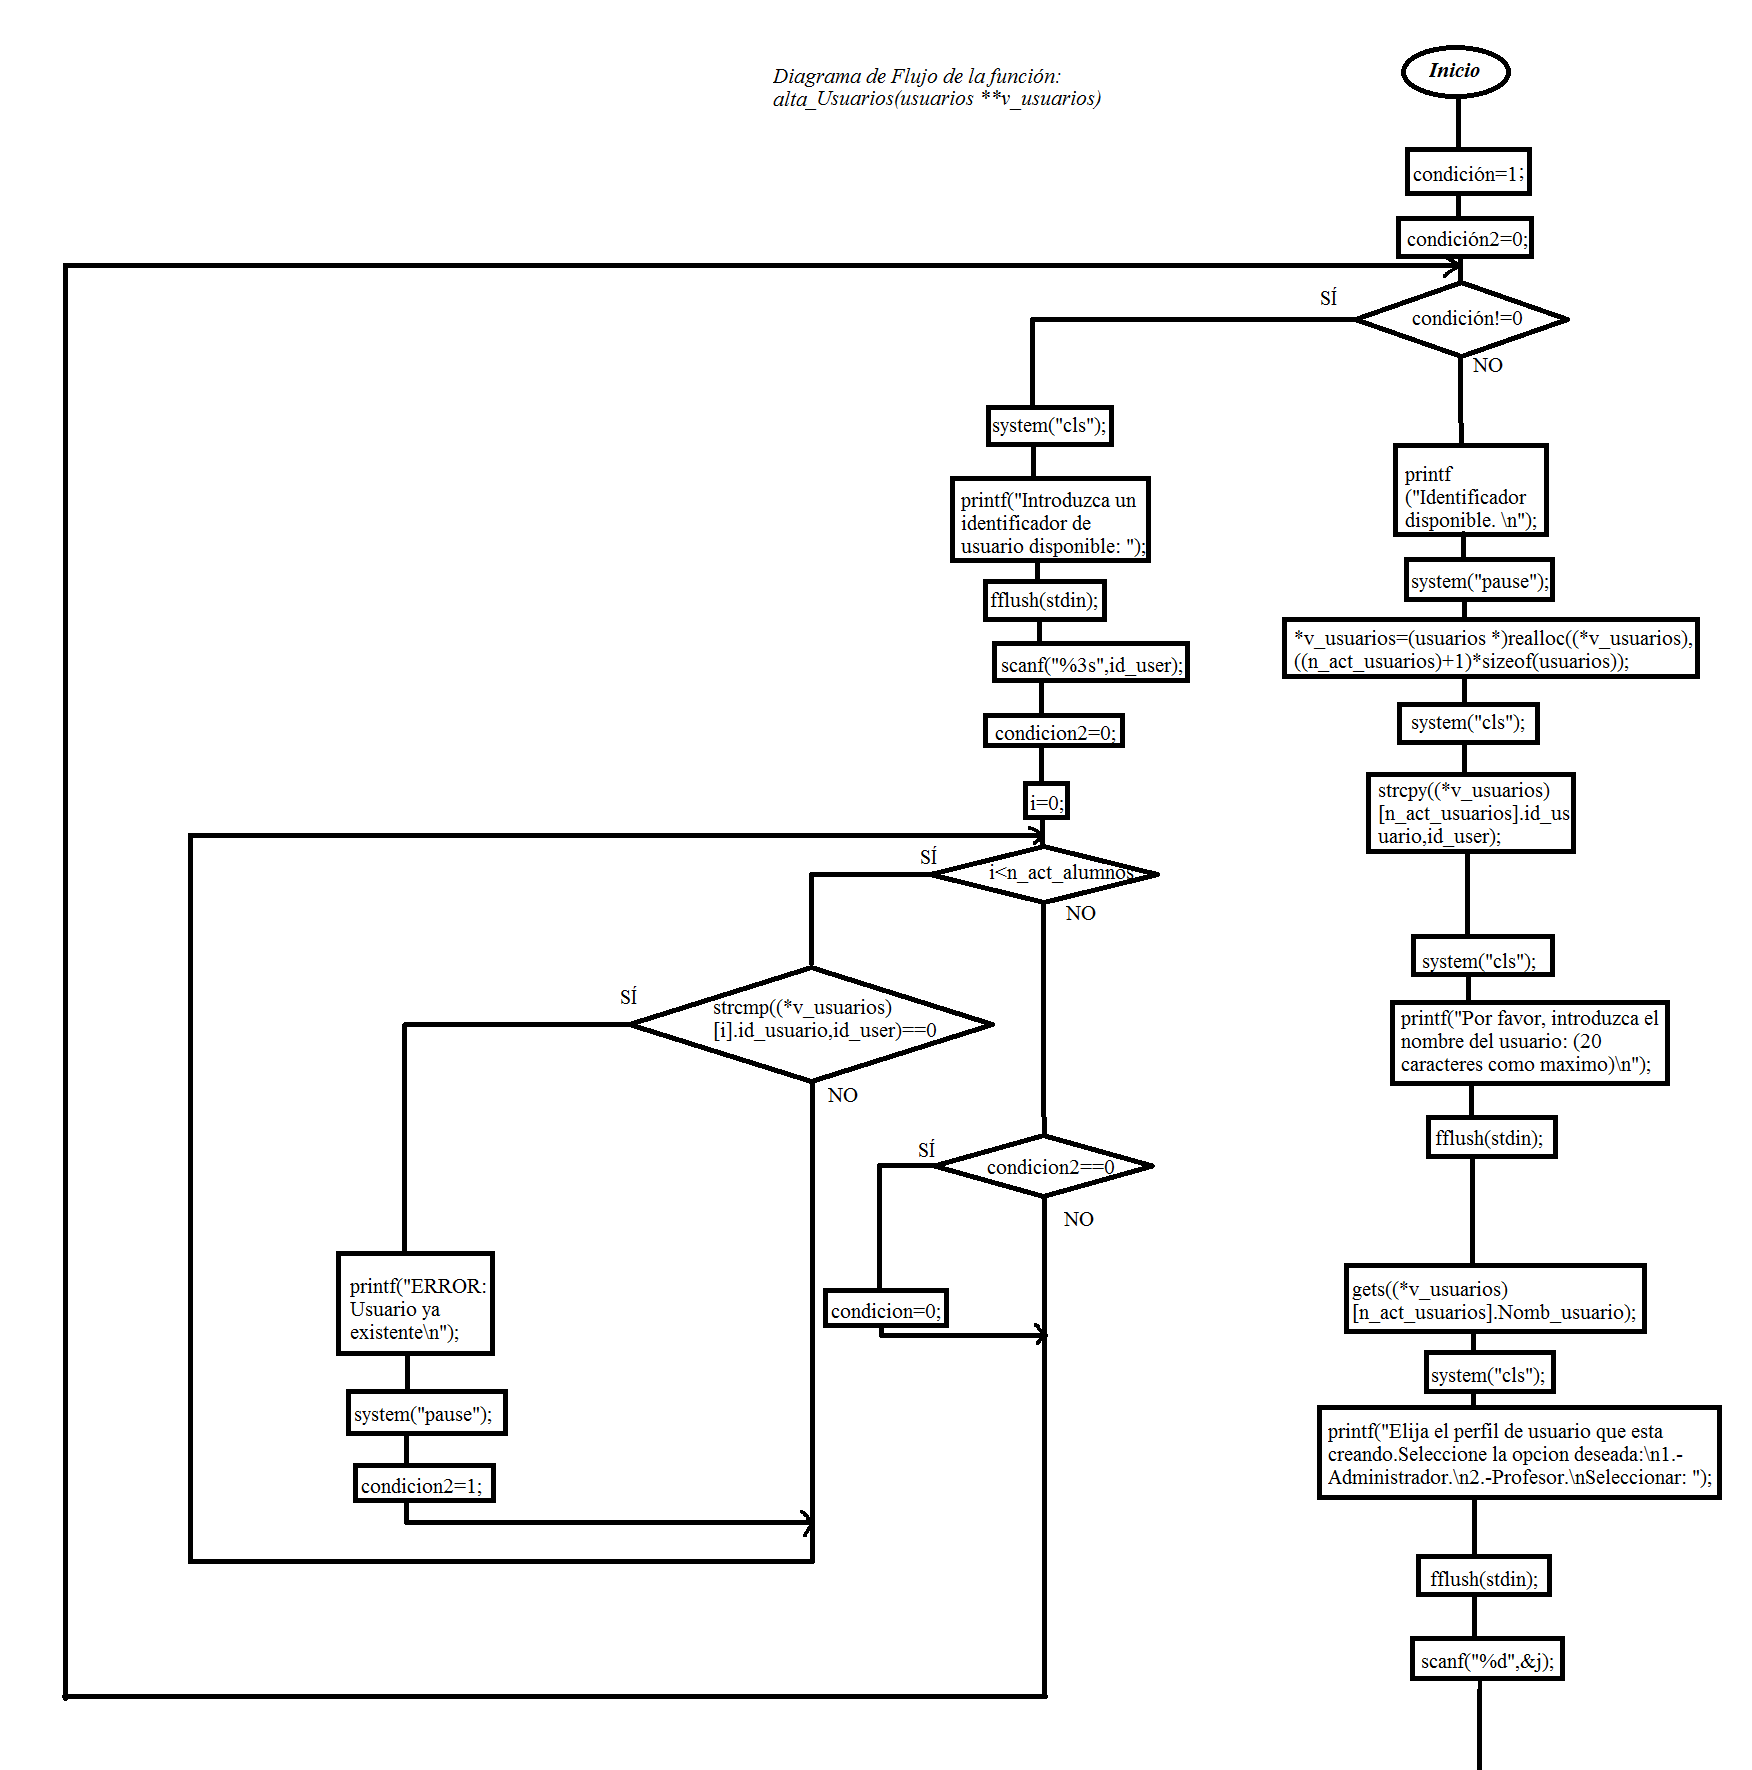
\includegraphics[scale=0.38]{CDF1.png}
\end{center}
\newpage
\begin{center}
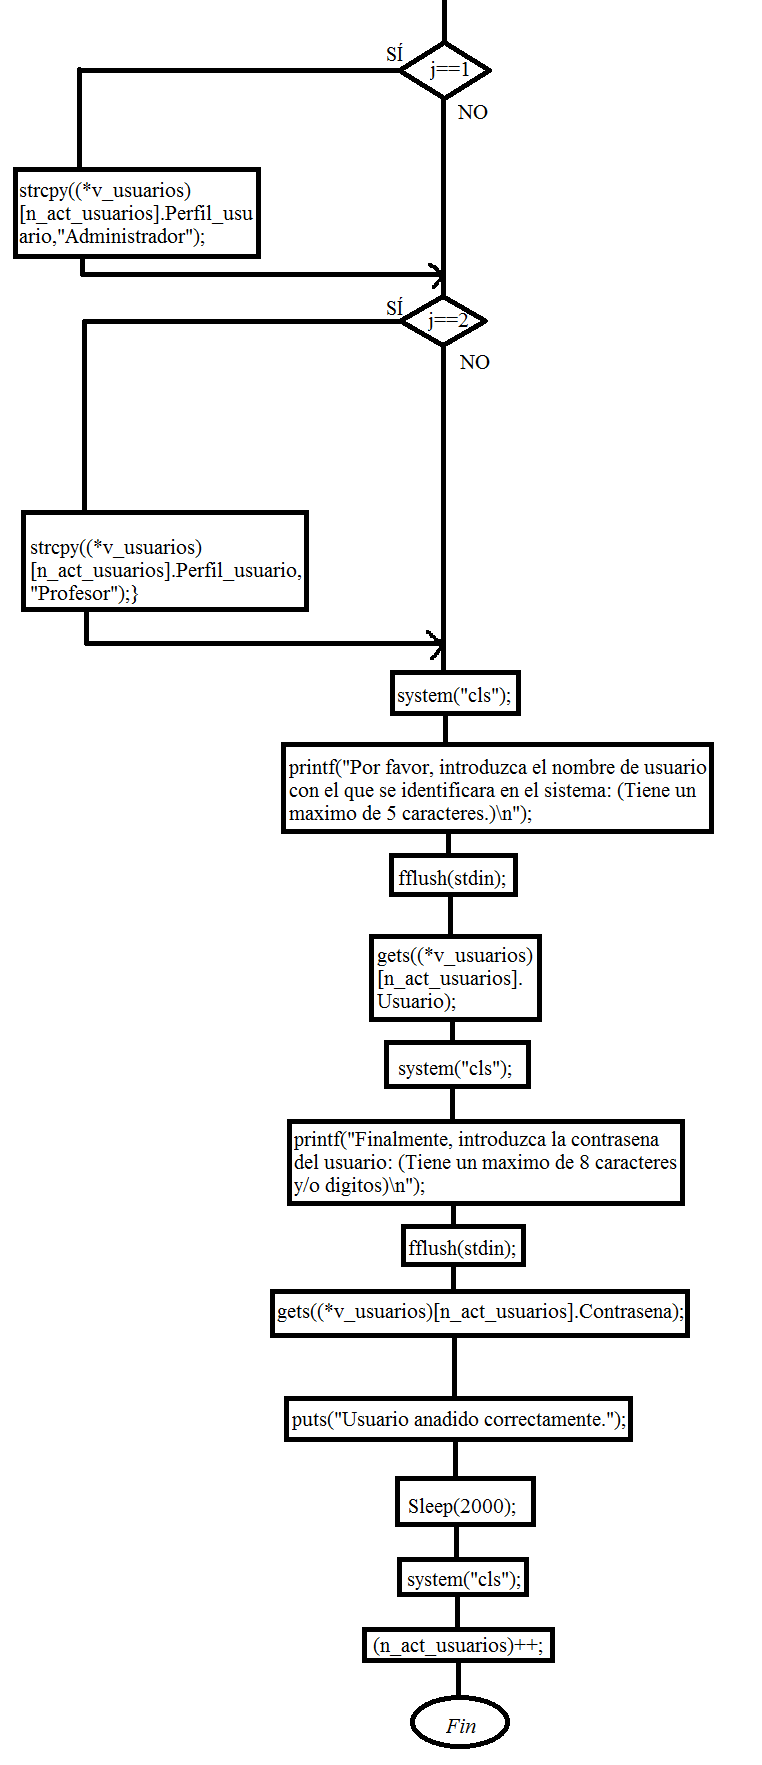
\includegraphics[scale=0.45]{CDF2.png}
\end{center}
\newpage
\subsubsection{Complejidad ciclomática}
\begin{center}
	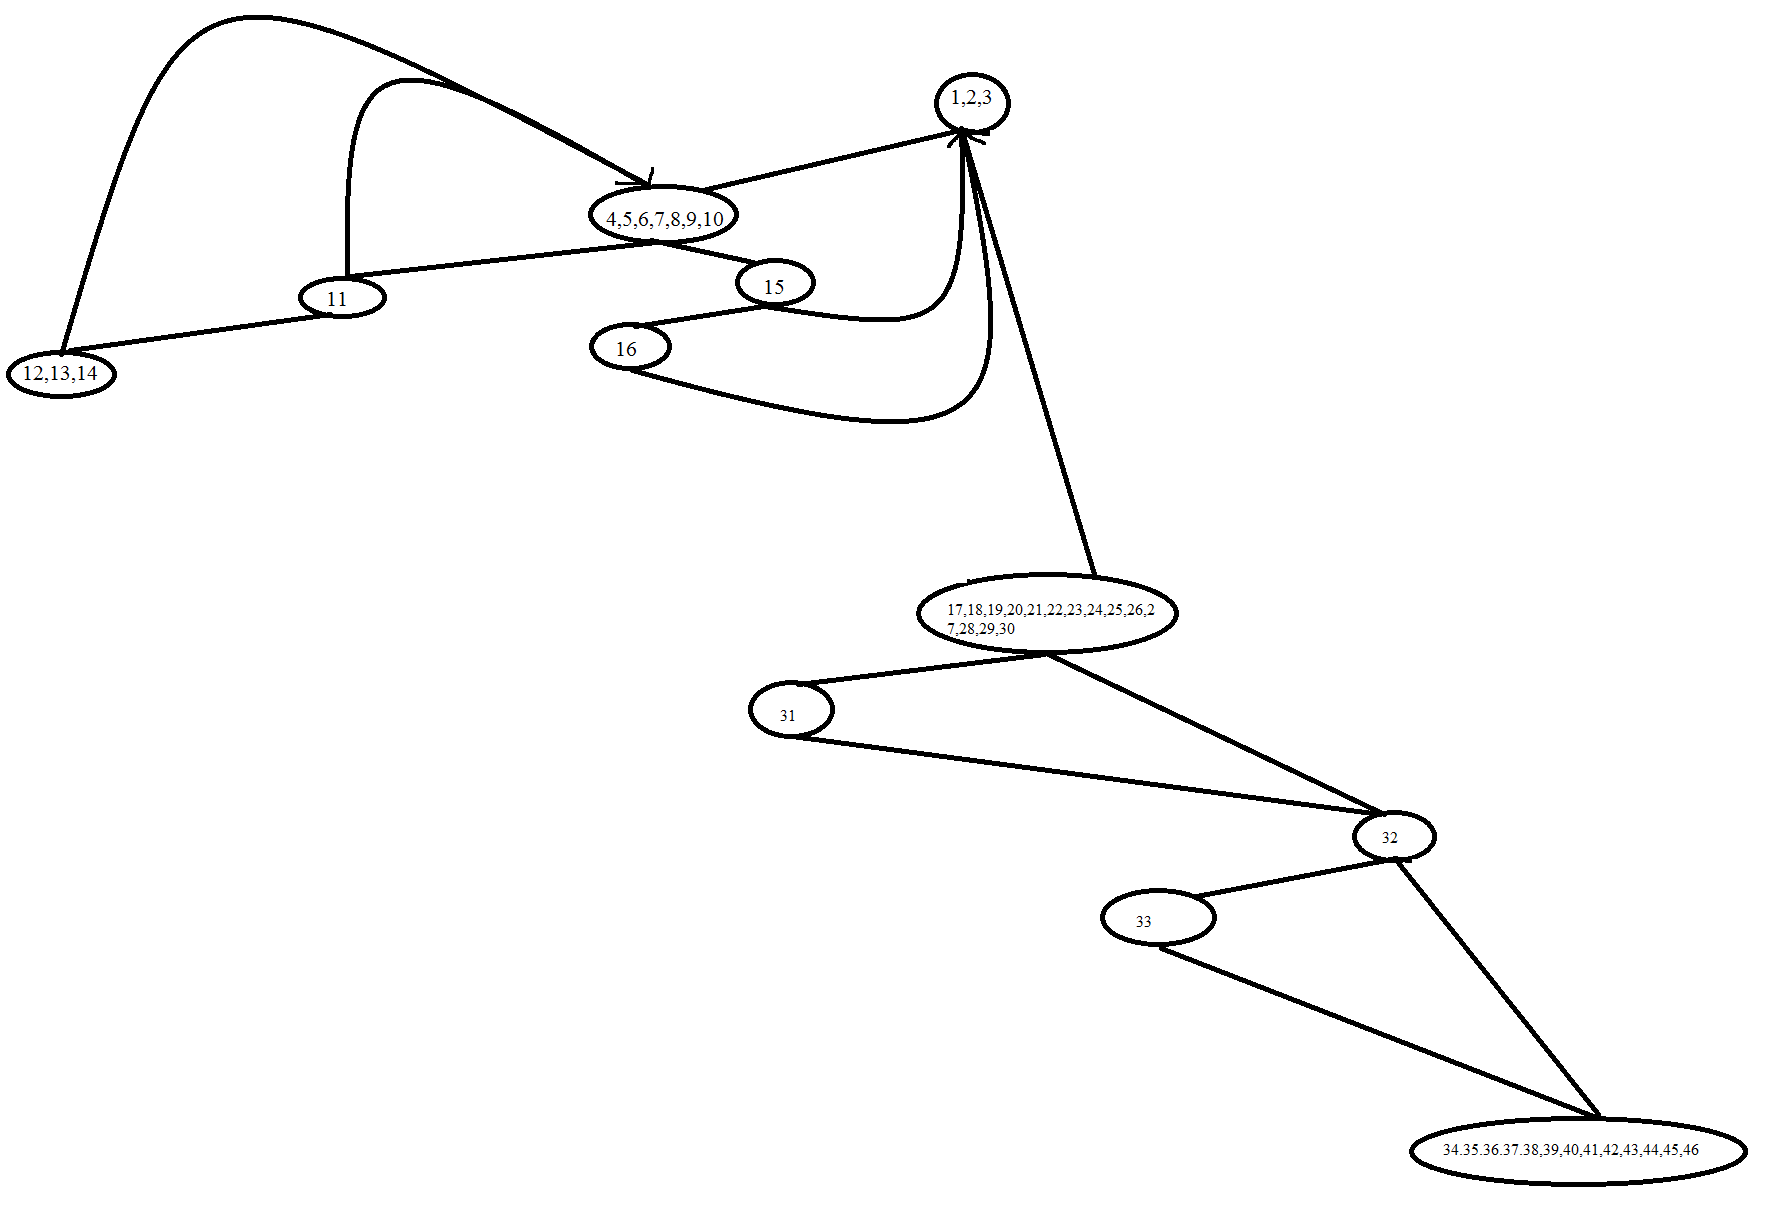
\includegraphics[scale=0.38]{ComplejidadCiclomatica.png}
\end{center}
La complejidad ciclomática se calcula de dos formas posibles:
\begin{itemize}
	\item $NA-NN+2$
	\item $NNP+1$
\end{itemize}
Siendo: NA el número de aristas, NN número de nodos y NNP número de nodos predicado (nodos que contienen alguna condición).\\
Para esta función tenemos:
\begin{itemize}
	\item $NA-NN+2 \Rightarrow 16-11+2=7$
	\item $NNP+1 \Rightarrow 6+1=7$
\end{itemize}
Por lo tanto, tenemos 7 posibles rutas que señalaremos con los números que indican los nodos de la complejidad ciclomática:
\begin{enumerate}
	\item 1, 2, 3, 17, 18, 19, 20, 21, 22, 23, 24, 25, 26, 27, 28, 29, 30, 32, 34, 35, 36, 37, 38, 39, 40, 41, 42, 43, 44, 45, 46.
	\item 1, 2, 3, 17, 18, 19, 20, 21, 22, 23, 24, 25, 26, 27, 28, 29, 30, 31, 32, 33, 34, 35, 36, 37, 38, 39, 40, 41, 42, 43, 44, 45, 46.
	\item 1, 2, 3, 4, 5, 6, 7, 8, 9, 10, 15, 1, 2, 3, 17, 18, 19, 20, 21, 22, 23, 24, 25, 26, 27, 28, 29, 30, 32, 34, 35, 36, 37, 38, 39, 40, 41, 42, 43, 44, 45, 46.
	\item 1, 2, 3, 17, 18, 19, 20, 21, 22, 23, 24, 25, 26, 27, 28, 29, 30, 32, 33, 34, 35, 36, 37, 38, 39, 40, 41, 42, 43, 44, 45, 46.
	\item 1, 2, 3, 4, 5, 6, 7, 8, 9, 10, 15, 16, 1, 2, 3, 17, 18, 19, 20, 21, 22, 23, 24, 25, 26, 27, 28, 29, 30, 32, 34, 35, 36, 37, 38, 39, 40, 41, 42, 43, 44, 45, 46.
	\item 1, 2, 3, 4, 5, 6, 7, 8, 9, 10, 11, 4, 5, 6, 7, 8, 9, 10, 15, 1, 2, 3, 17, 18, 19, 20, 21, 22, 23, 24, 25, 26, 27, 28, 29, 30, 32, 34, 35, 36, 37, 38, 39, 40, 41, 42, 43, 44, 45, 46.
	\item 1, 2, 3, 4, 5, 6, 7, 8, 9, 10, 11, 12, 13, 14, 1, 2, 3, 17, 18, 19, 20, 21, 22, 23, 24, 25, 26, 27, 28, 29, 30, 32, 37, 38, 39, 40, 41, 42, 43, 44, 45, 46.
	
	
\end{enumerate}

\section{Pruebas de caja negra}
Las pruebas de caja negra se realizan para determinar que cada función realiza la tarea para la que ha sido creada. Por lo tanto, se analiza la especificación de las funciones, su entrada y su salida.\\
En la función que estamos tratando (\texttt{alta\_Usuarios}), podemos ver que en la precondición nos pide que el vector \texttt{v\_usuarios} tiene que estar inicializado antes de realizar la llamada a esta función.\\
En su postcondición se establece su funcionalidad: creará un nuevo usuario en el sistema añadiendo una nueva posición al vector \texttt{v\_usuarios}.\\
Diferentes casos de prueba a tener en cuenta:
\begin{itemize}
	\item Si en la sentencia \texttt{if} de la línea 21 de código se cumple la condición, el programa habrá encontrado un usuario que tiene el mismo identificador que el que queremos introducir, por lo tanto, abortará la tarea de dar de alta un nuevo usuario y volverá a pedir un nuevo identificador. Si esta sentencia no se cumple, el programa continuará con el alta del usuario.
	\item El bucle de la línea 19 de código sirve para recorrer el vector de posiciones buscando un usuario que tenga el mismo identificador que el que hemos introducido por teclado. Cuando llegue al valor de la variable \texttt{n\_act\_usuarios} terminará el recorrido continuando con la siguiente sentencia condicional \texttt{if} de la línea 27.
	\item La sentencia condicional \texttt{if} de la línea 27 de código establece la condición de haber encontrado un usuario con el mismo identificador y establecerá a 0 la variable \texttt{condicion} en caso de no haber encontrado dicho usuario.
	\item El bucle más externo se encuentra en la línea 13 de código que es el que se encarga de controlar toda la gestión de la introducción del usuario de un identificador válido e inexistente en el sistema. Si no se introduce un identificador válido, lo seguirá exigiendo hasta que se le introduzca.
	\item Por último en las líneas 55 y 57 se encuentran dos sentencias condicionales que se encargan de fijar el rol que representarán los usuarios en el sistema, que será seleccionado en el registro de cada uno de ellos. Si se elige la opción ``1'' será un administrador y si se elige la opción ``2'' será un profesor.
\end{itemize}

\end{document}
